\documentclass{article}
\usepackage[utf8]{inputenc}
\usepackage[T1]{fontenc}
\usepackage{amsmath}
\usepackage{graphicx}
\usepackage{amssymb}
\usepackage{float}
\usepackage{tikz}
\usepackage{pgfplots}
\usepackage[letterpaper, margin=1in]{geometry}
\usepackage{hyperref}
\hypersetup{
	colorlinks=true,
	linkcolor=blue,
	citecolor=blue,
	filecolor=blue,      
	urlcolor=blue,
	pdftitle={Concealed Bike Anti-Theft Device},
	pdfpagemode=FullScreen,
}


\begin{document}

\begin{titlepage}
	\title{Concealed Bike Anti-Theft Device: Design Document}
	\author{Elizabeth Atkinson (eatkinso)\\ Srinidhi Raman (nidhim2) \\ Alex Wen (acwen2) }
\end{titlepage}



\maketitle{}

\tableofcontents


\section{Introduction}
\subsection{Problem}

\paragraph{}
College students frequently face the issue of bikes being stolen on campus. Even with the strongest of protections, they are not completely capable of deterring thieves who have various equipment. Our own member, Elizabeth, had her bike secured with a substantial solid steel U-lock, but was stolen regardless last fall, when someone apparently sawed through the u-lock at night. 

In order to discourage bike theft, it would be useful to have a bike anti-theft device that could enable the user to track the bike's location wirelessly. 

\subsection{Solution Overview}
\paragraph{}
We propose a concealed bike anti-theft device that helps bikers prevent their bike from being stolen by unlocking to a specific RFID key (therefore difficult to mimic), providing GPS tracking so the user has the ability to track down the bike if stolen, and frightening away potential thieves with a loud noise when theft is detected.

The device will receive GPS coordinates and periodically transmit the coordinates over LoRa to be received by the user. To allow the bike system to differentiate between potential thieves and the owner, the owner of the bike will have an RFID tag such that while the user is on the bike, the RFID tag can be detected. \begin{abstract}
	
\end{abstract}
If the bicycle is moved when the RFID tag is not nearby, it will trigger a loud and annoying alarm to scare away the potential thief.

The device will be designed in a manner such that it is difficult to find and remove, discouraging potential bike thieves from removing the bike. Additionally, the device will be designed to fit a relatively universal bike structure, which will allow the device to be attached to any bike. A standardized device will be more convenient for users as bikes with integrated tracking systems tend to be very expensive.

Our device will be small, rechargeable, battery-powered, and enclosed in a weatherproof enclosure that can easily be attached to most bikes.
\subsection{High-Level Requirements}

\begin{enumerate}
	\item If a user tries to remove the bike from a stationary location without the RFID tag, the alarm will sound. 
	
	\item The device receives GPS data \textit{at least} once per minute, and records its own position over time.  
	
	\item The device transmits its GPS location data and additional data over LoRa to be received by a base station. 
	
\end{enumerate}

\section{Design}
\subsection{Conceptual Visual Aid} 

\begin{figure}[H]
	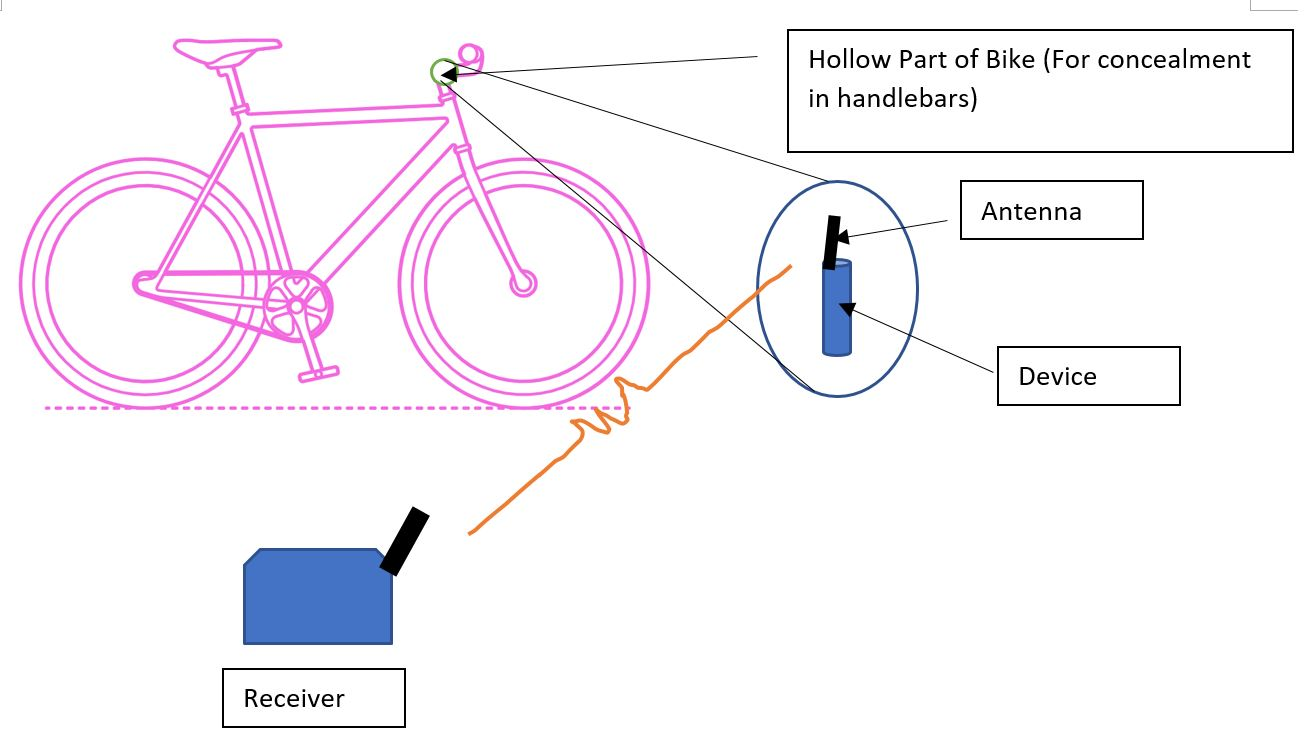
\includegraphics[width=\textwidth]{visual_aid.JPG}
	\caption{Conceptual Diagram}
\end{figure}


\subsection{Overall System Block Diagram}
\begin{figure}[H]
	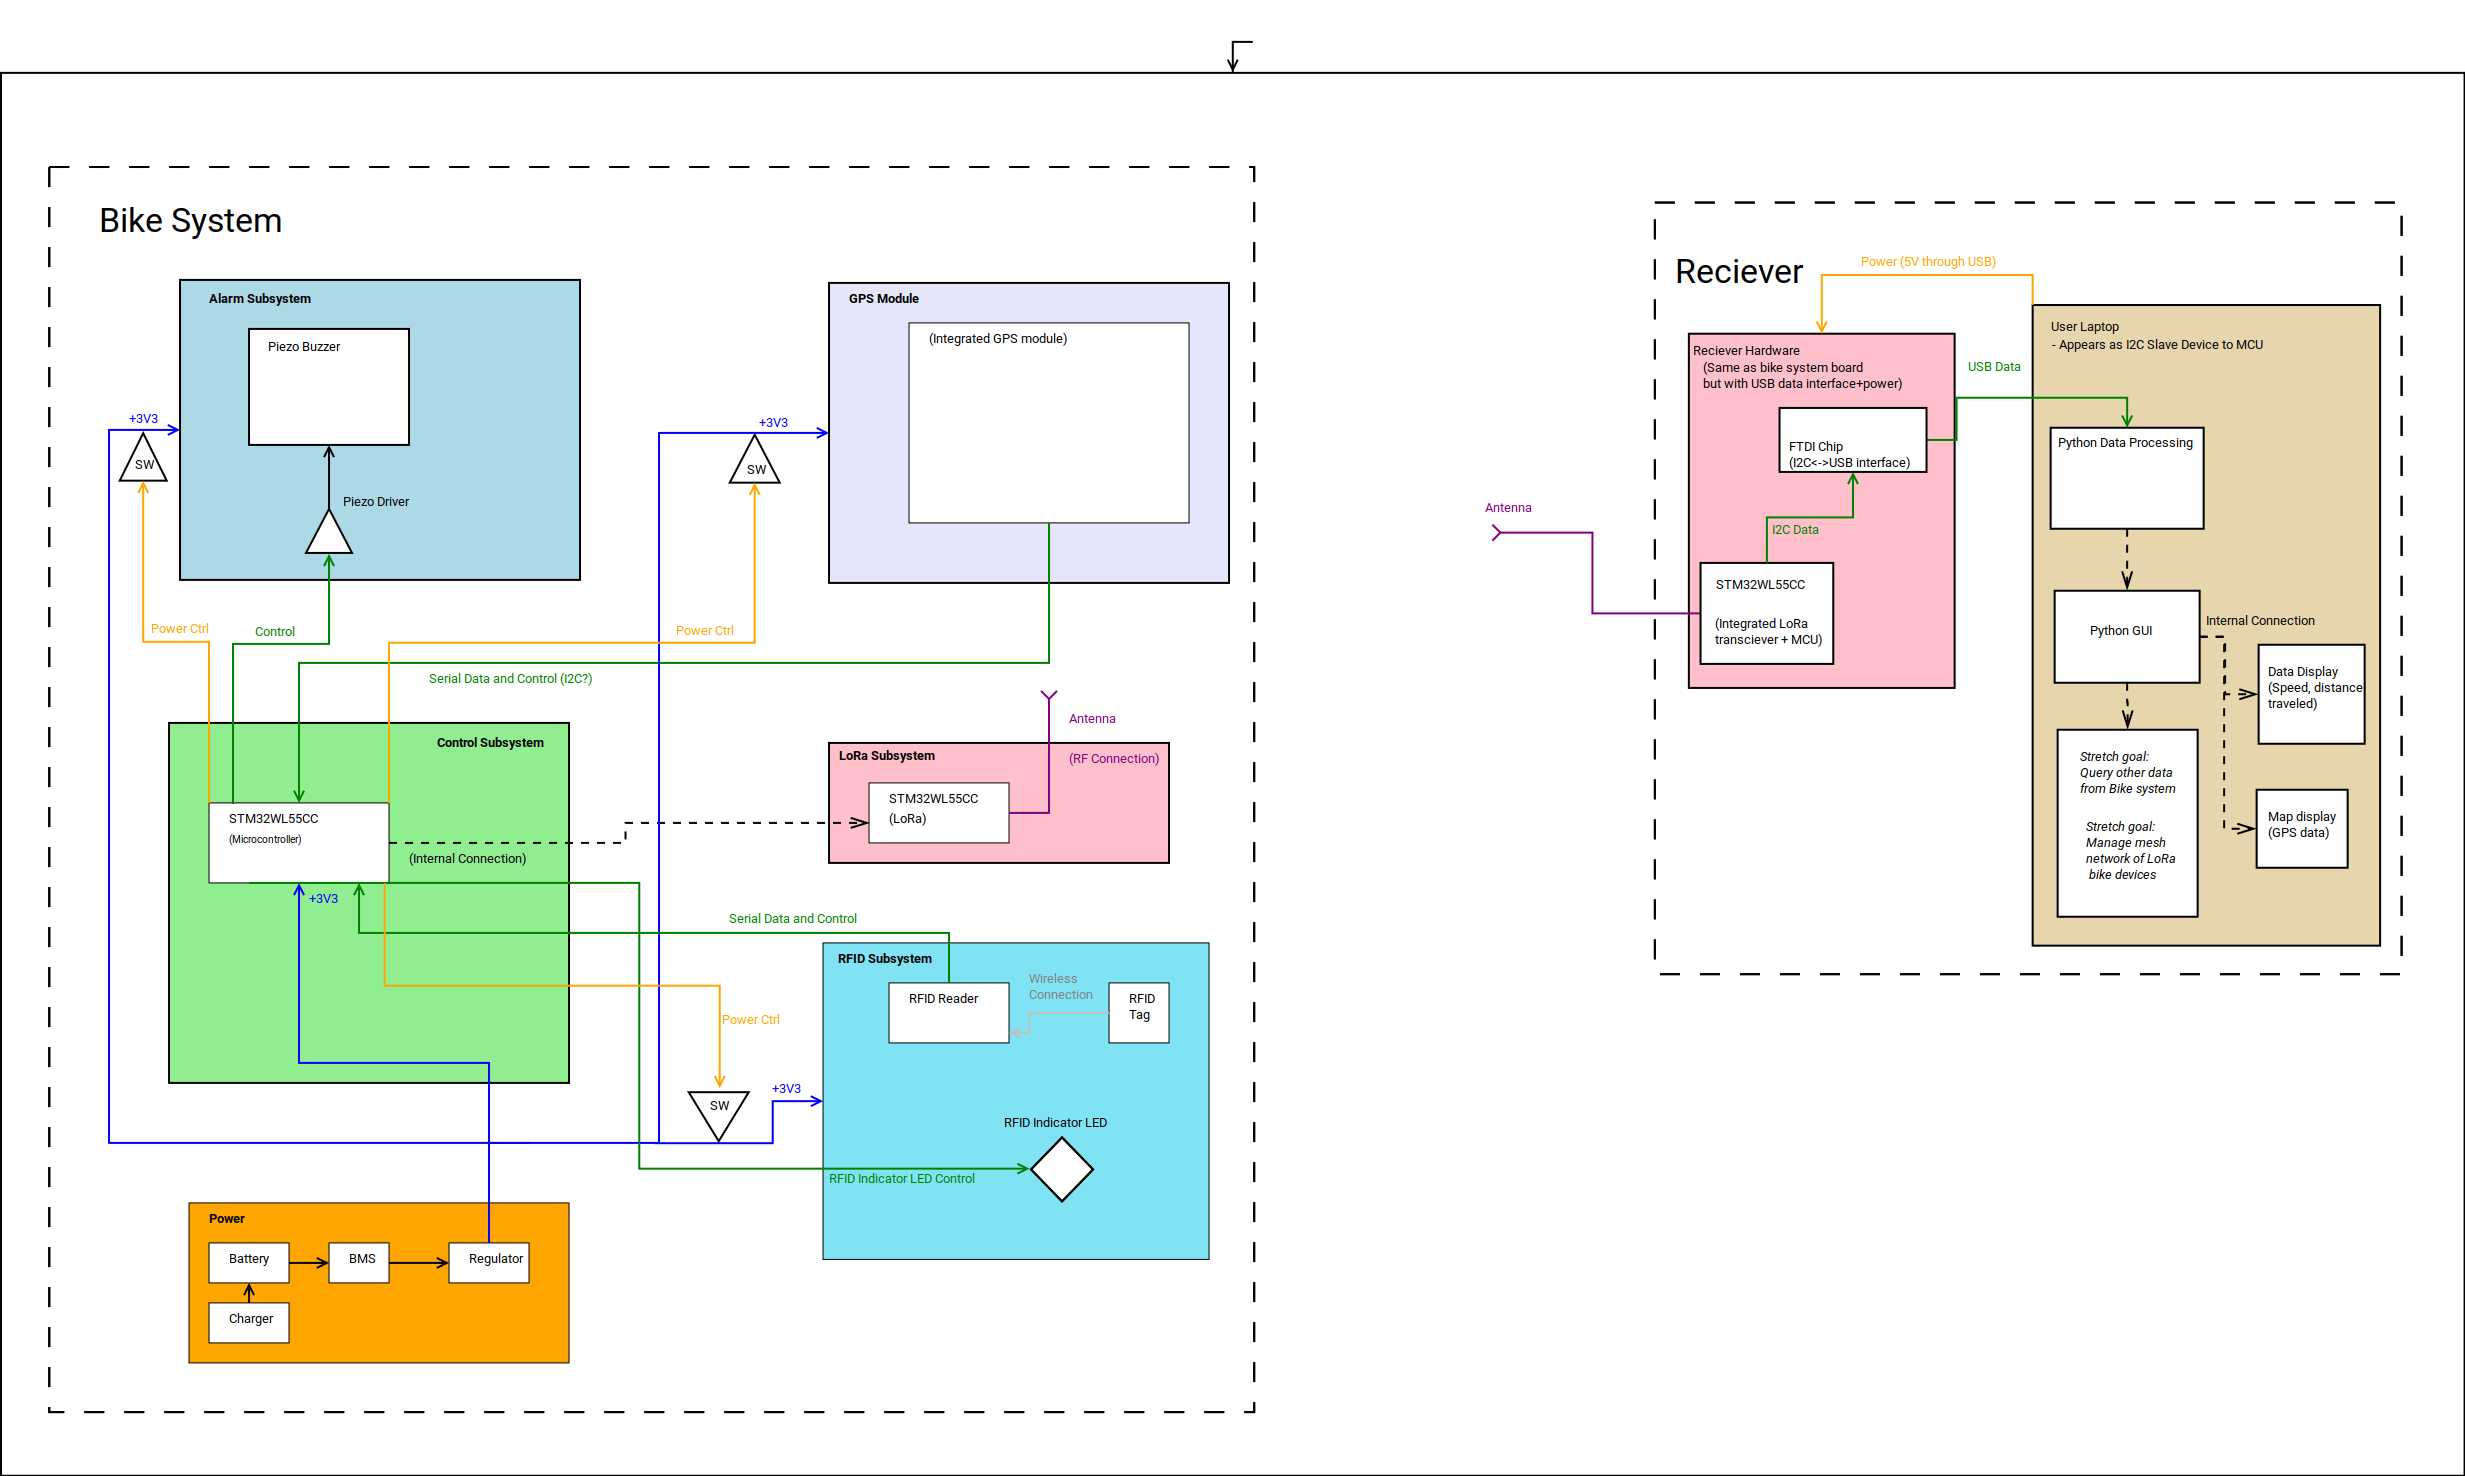
\includegraphics[width=\textwidth]{block_diagram_full.png}
	\caption{Full Block Diagram}
\end{figure}


\subsection{Physical Design}

\subsection{Subsystem Designs} 
\subsubsection{On-Bike Control System}

\paragraph{}
We will use the STM32WL55CC, an SoC that includes both a dual-core ARM microcontroller and a wireless transceiver \cite{stm_datasheet}. The microcontroller will be responsible for buffering data from the GPS receiver, packetizing the data to send over LoRa, and internally transferring the data to the integrated RF transceiver. The microcontroller will also manage the control signals for the alarm subsystem, RFID subsystem, and GPS module. 

Since this is a battery-powered device, the microcontroller will also be responsible for implementing power-saving measures. For example, the microcontroller will vary the number of GPS data transmissions depending on the bike state: while the bike is in a “idle/safe” state (stationary in one location) it will only transmit its location over LoRa once per hour. If the device is in the “stolen” state, it will transmit its location over LoRa once per minute. The microcontroller will also cut off power to the Alarm when it is not in use, and as a stretch goal, the microcontroller will selectively cut power to the RFID/GPS subsystems in an intelligent manner (ie, the RFID transmitter will not continuously transmit/listen for the RFID tag if the GPS module detects that the bike is in motion, and the motion was initiated by the correct user). 
\paragraph{} 

\begin{figure}[H]
	\begin{centering}
	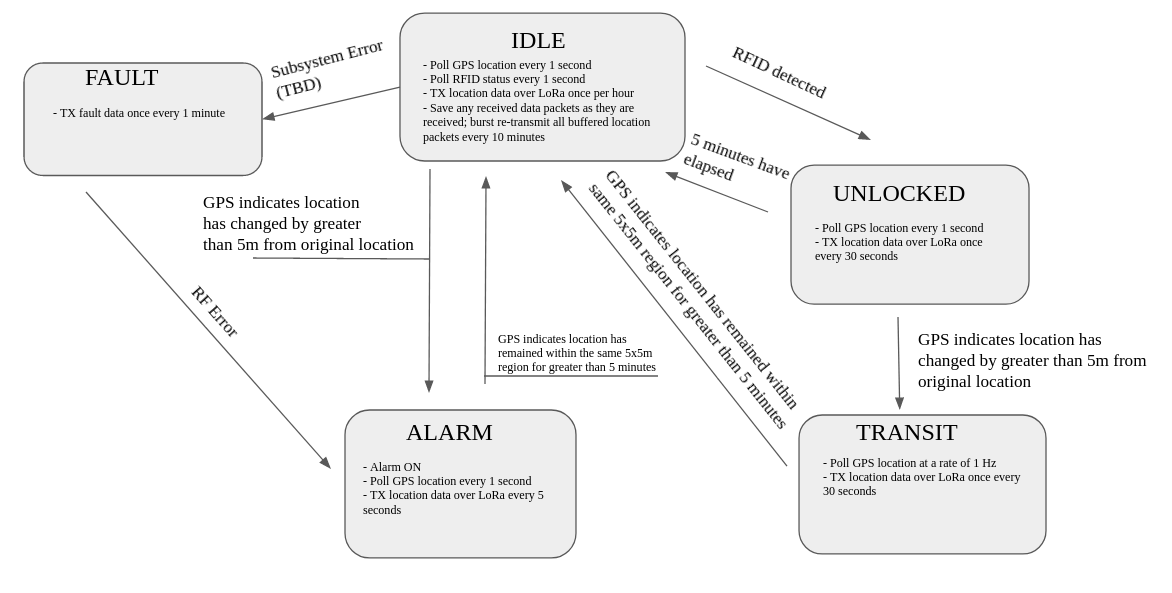
\includegraphics[width=\textwidth]{state.png}
	\caption{Control System State Machine}\label{state}
	\end{centering}
\end{figure}

\begin{figure}[H]
	\begin{centering}
	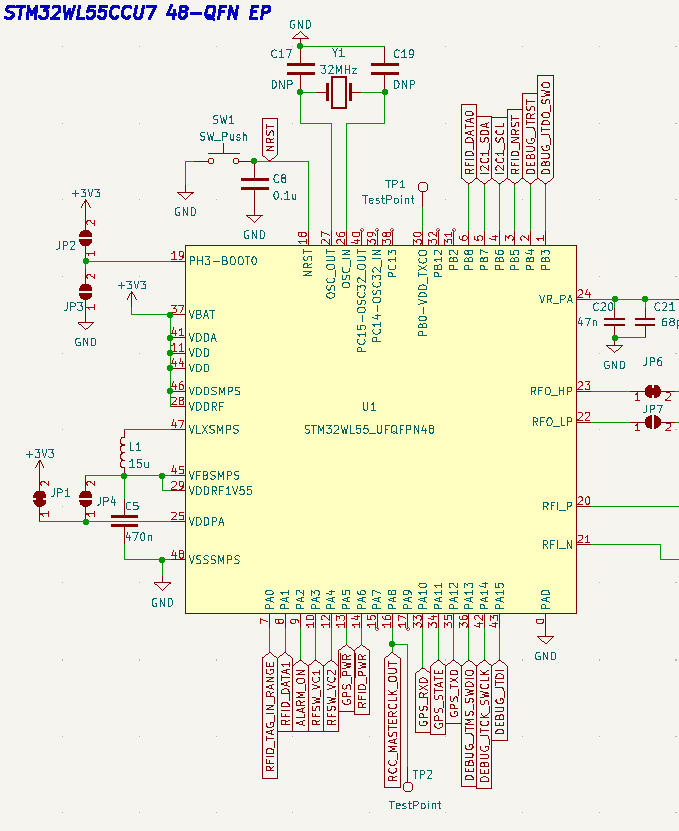
\includegraphics[width=0.5\textwidth]{mcu_schematic.png}
	\caption{Microcontroller and Support Circuitry Schematic}
	\end{centering}
\end{figure}

\textit{\textbf{Control Subsystem Requirements \& Verification}}


\begin{figure}[H]
	\begin{center}
		\begin{tabular}{|p{0.3 \linewidth}|p{0.6 \linewidth}|}
			\hline
			Requirement & Verification  \\
			\hline
			\begin{enumerate}
				\item  The microcontroller implements a state-based control system with power-saving measures in the idle/safe states.  
			\end{enumerate} &
		\begin{enumerate}
			\item Flash the firmware to the device. 
			\item Monitor the state transitions during device operation. 
		\end{enumerate}  \\
			\hline
			\begin{enumerate}
				\item The microcontroller packetizes data to be sent over LoRa at the update rate specified by the state diagram in figure \ref{state}.
			\end{enumerate} & \begin{enumerate}
			\item Flash test firmware that cycles through each of the states. 
			\item Verify that the TX update rate is greater than once per hour in the IDLE, UNLOCK, and TRANSIT states. 
		\end{enumerate} \\
			\hline 
		\end{tabular}
	\end{center}
	\caption{Microcontroller R\&V Table.}
\end{figure}



\subsubsection{LoRa Subsystem}

\paragraph{} We will use LoRa, a low-power spread-spectrum RF protocol, to transmit GPS data from the bike device to be received by the user. LoRa is an ideal choice for this application because it is extremely low-power, has a range of several miles even in crowded city conditions, and does not require any radio licensing to operate \cite{LoRA}. These qualities will enable our device to function for extended periods of time on battery power, allow the signal to be received by the base station for multiple miles, and allow any user to purchase this device and use it without worrying about licensing. 


The LoRa transceiver is integrated with the STM32WL55CC SoC, so the LoRa subsystem will require us to design an external matching network and antenna \cite{matchingAN}. We will use the ST RF design guide to design an appropriate matching network, and we will verify that the RF network will not cause damage to the device prior to populating the STM32. We will choose a compact antenna and conceal it to prevent theft (for example, inside a hollow conventional plastic reflector that can be mounted on the handlebars or seat; refer to figure \ref{reflector} for an example of one type of bike reflector). 

As a stretch goal, we will implement a rudimentary form of mesh networking between bike tracking devices. Each bike tracker will listen and re-transmit GPS coordinates it receives from other bike trackers -- as a result, the range of the LoRa bike tracker will be dramatically increased, since its GPS coordinates can be received as long as \textit{any} bike tracker is in range instead of only if the base station is in range. 
\paragraph{} 

\begin{figure}[H]
	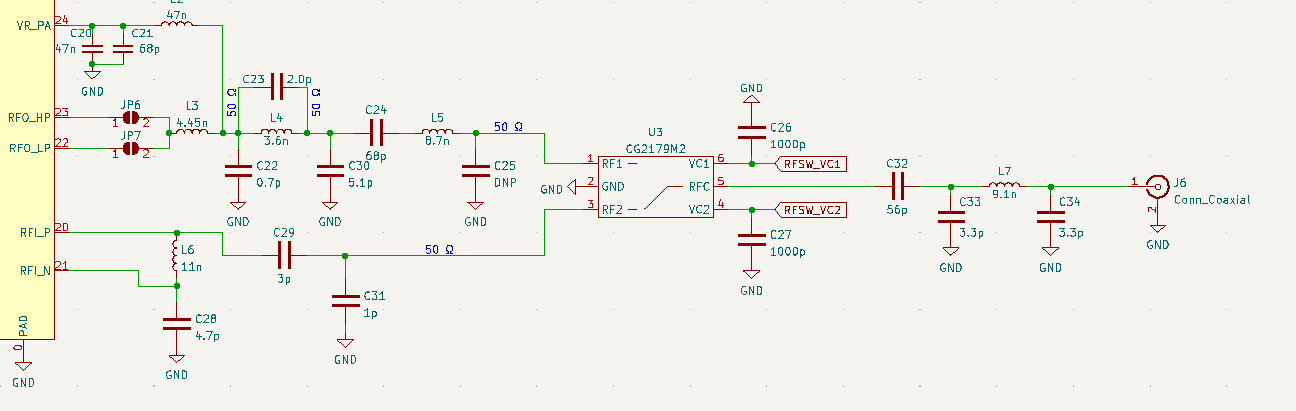
\includegraphics[width=\textwidth]{rf-ckt.png}
	\caption{RF Matching and Filtering Network Schematic} \label{rf-sch}
\end{figure}


\textit{\textbf{LoRa Subsystem Requirements and Verification:}}

\begin{figure}[H]
	\begin{center}
		\begin{tabular}{|p{0.3 \linewidth}|p{0.6 \linewidth}|}
			\hline
			Requirement & Verification  \\
			\hline
			\begin{enumerate}
				\item The LoRa subsystem matching network and antenna have a VSWR of less than 10 at the RF output of the STM32WL55CC. 
			\end{enumerate}  & \begin{enumerate} 
			\item Populate the RF matching network before populating the microcontroller.
			\item Calibrate the VNA from 800-1200 MHz with PCB TRL standards. 
			\item Terminate the SMA output of the PCB with a 50 ohm load.
			\item Measure the input impedance looking into the RF matching network at the RF output of the STM32WL55CC.
			\item Calculate the VSWR from the measured input impedance and the specified PA output impedance in the STM32 datasheet. 
			\end{enumerate}
			 \\
			\hline
			\begin{enumerate}
				\item The antenna is hidden in a common bike component such as a reflector so that it is not visibly obvious. 
			\end{enumerate}  & \begin{enumerate}
			\item Objective visual verification. 
			\item Ask other senior design students.
		\end{enumerate} \\
			\hline
		\end{tabular}
	\end{center}
	\caption{LoRa Subsystem R\&V Table.}
\end{figure}


\subsubsection{GPS Module}
\paragraph{} 
We will use an off-the-shelf GPS module to receive GPS data. We will choose a GPS module that can receive GPS updates at a rate of at least 1 Hz. We will mount the GPS module on the bike such that the GPS antenna is able to see a clear view of the sky, but is concealed from the casual observer. We will likely conceal the small patch antenna inside of a plastic bike reflector such as the type shown below. \footnote{We are not sure if bike reflectors have metal foil inside the plastic -- if this is the case we will obviously remove the metal foil before mounting the antenna.} Since the GPS module is a PCB with antenna and connector, we will not need to make a carrier board, we will only need to provide the appropriate connector for data, power and control. 

\begin{center}
	\begin{figure}[H]
		\centering
		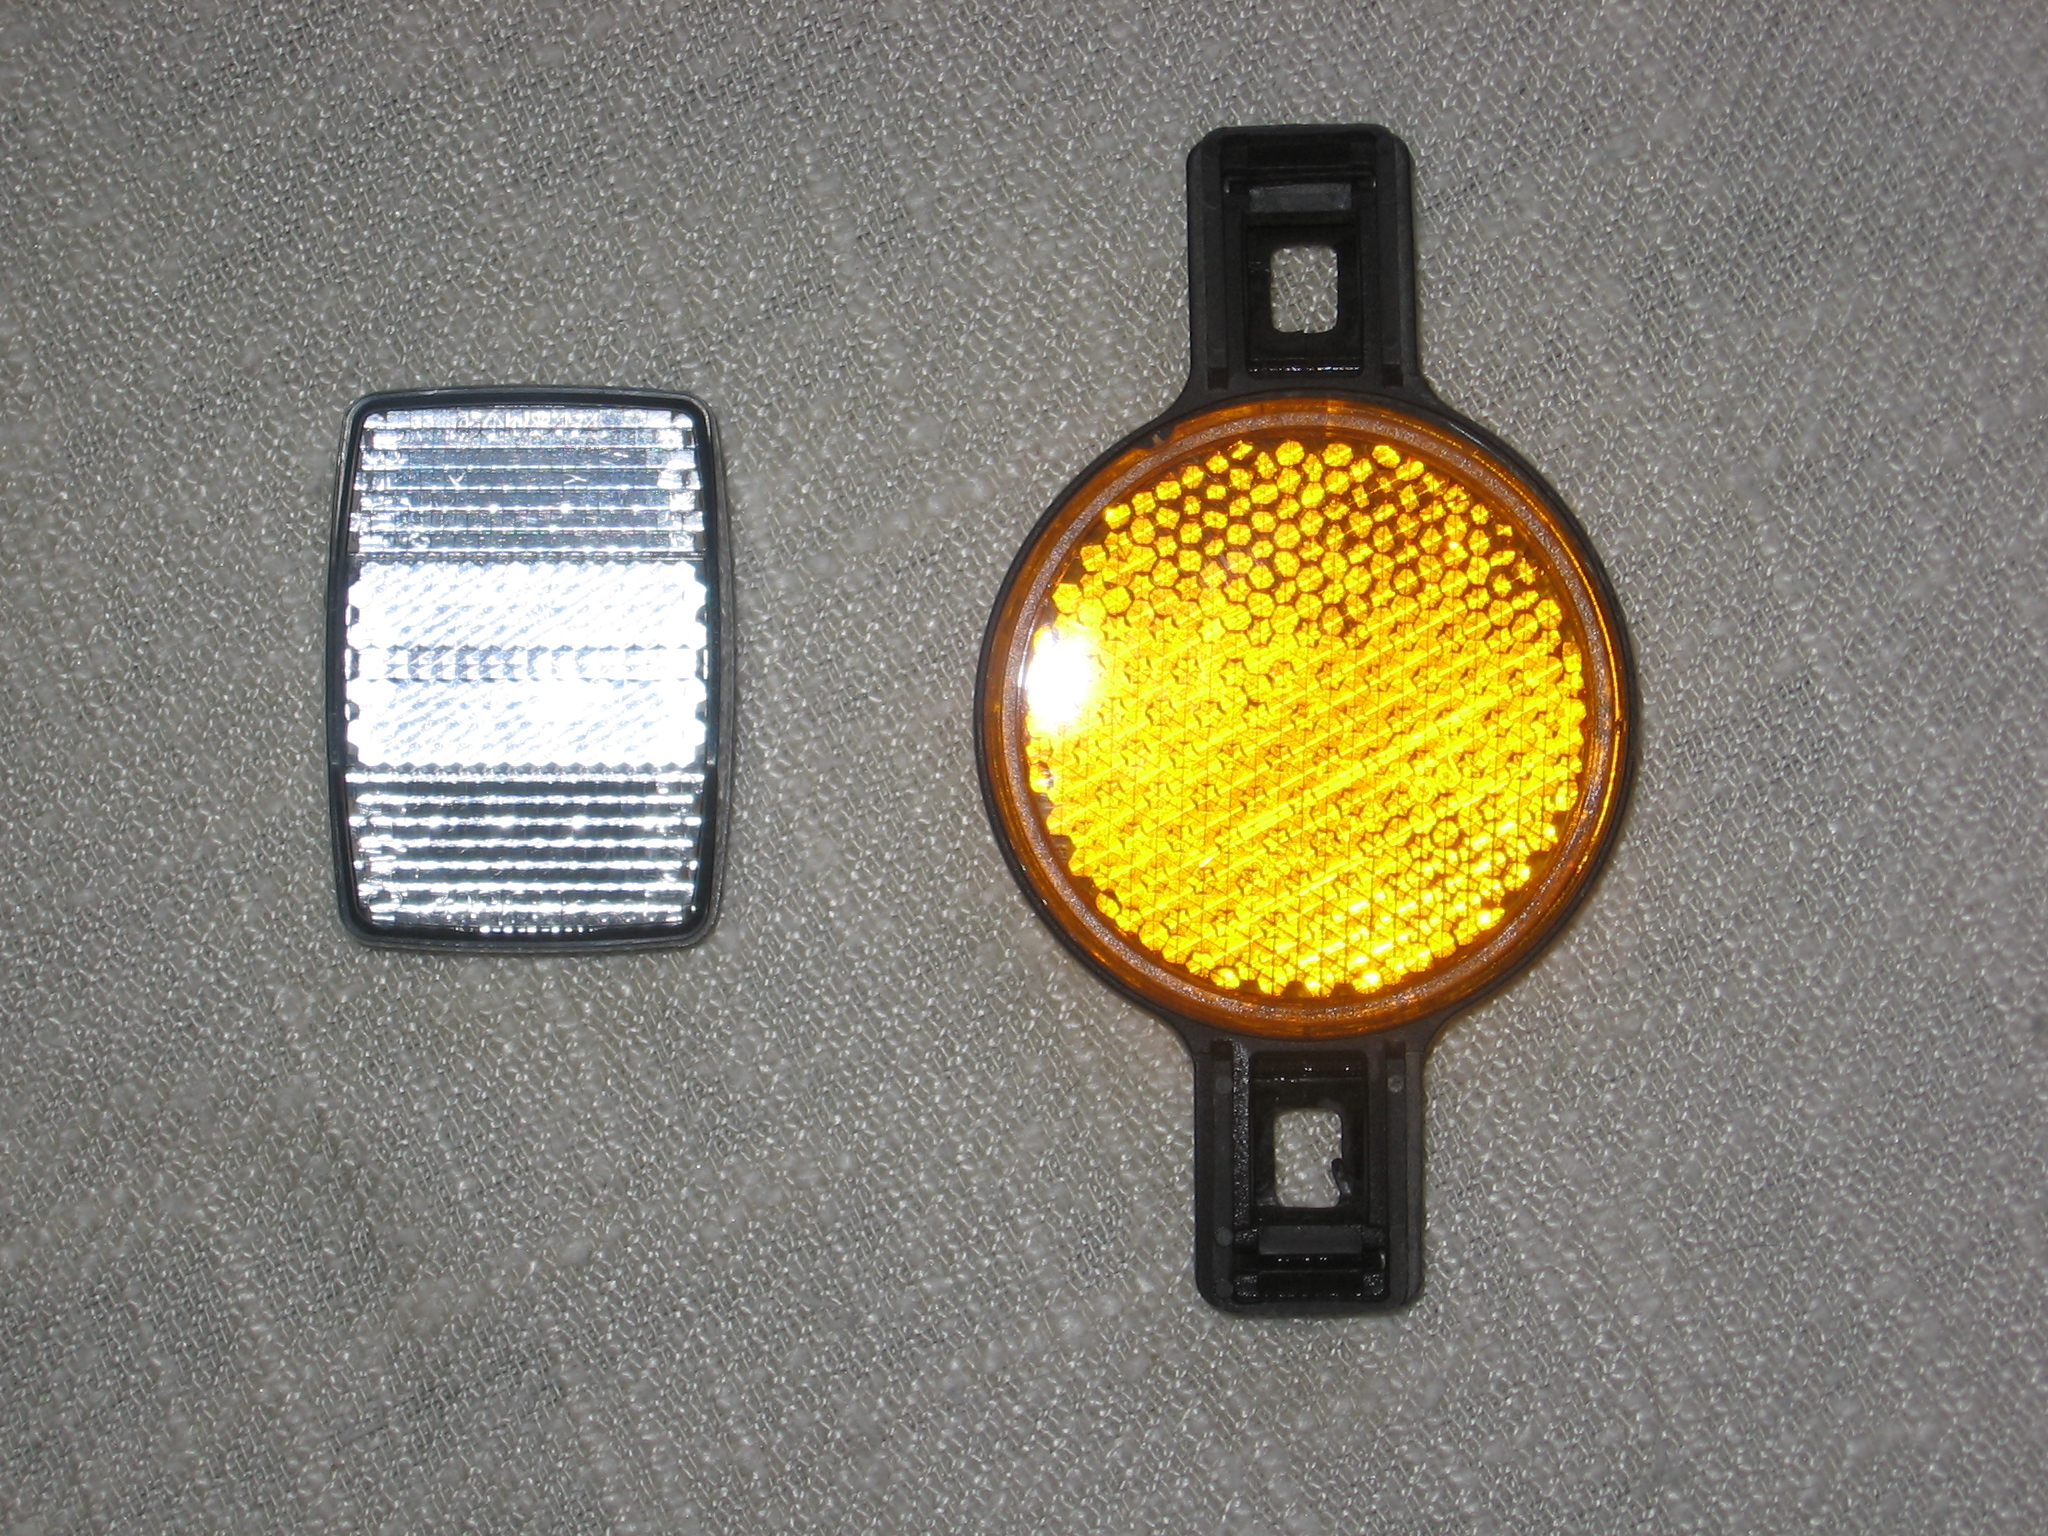
\includegraphics[width=0.25 \textwidth]{bike_reflector.jpg}
		\caption{Example of a plastic bike reflector.} \label{reflector}
	\end{figure}
\end{center}


\paragraph{} 


\textit{\textbf{GPS Subsystem Requirements:}}

\begin{enumerate}
	\item The GPS module can communicate with the microcontroller at a update rate of greater than 1 Hz. 
\end{enumerate}	


\begin{figure}[H]
	\begin{center}
		\begin{tabular}{|p{0.3 \linewidth}|p{0.6 \linewidth}|}
			\hline
			Requirement & Verification  \\
			\hline
			\begin{enumerate}
				\item   The GPS module can communicate with the microcontroller at a update rate of greater than 1 Hz.  
			\end{enumerate} &
			\begin{enumerate}
				\item  Flash a test program to the microcontroller that continuously polls the GPS module.
				\item Verify that the GPS module transfers GPS data at an update rate of greater than 1 Hz.
			\end{enumerate}  \\
			\hline 
		\end{tabular}
	\end{center}
	\caption{Microcontroller R\&V Table.}
\end{figure}

\subsubsection{RFID Subsystem}


\paragraph{} We will use an off-the-shelf RFID tag and an RFID reader module. The RFID module will listen to determine if the bike owner's RFID tag is present, and transfer the RFID data to the microcontroller. The microcontroller must be able to read the RFID identifier from the transferred data to determine if the owner's RFID tag is present (so that the device does not just trigger when any RFID is present). 

To increase ease of use, we will include a visual indicator such as a concealed LED to show whether or not the correct RFID tag has been detected so that the user doesn't accidentally set off the alarm. The visual indicator will be concealed in a common bike component or unobtrusive location. 


We will wind a coil to be used as the antenna for the RFID detector; we will use the design guidelines in \cite{rfid} to make an appropriate coil. 



\begin{center}
	\begin{figure}[H]
		\centering
		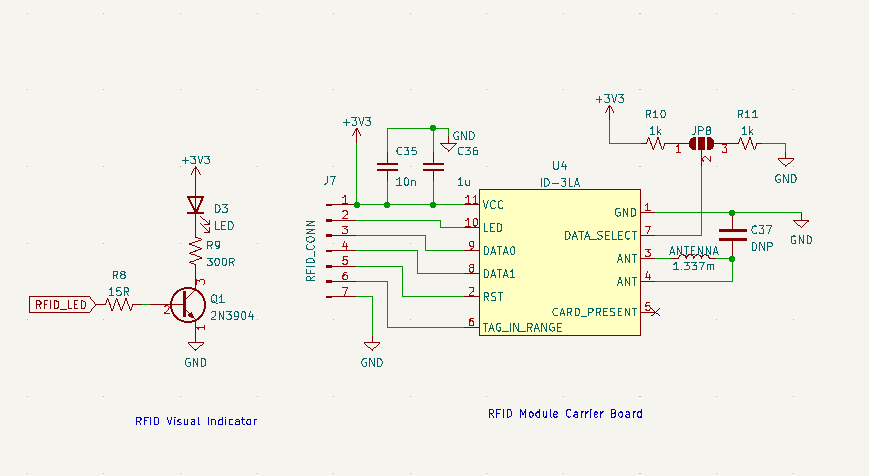
\includegraphics[width= \textwidth]{rfid_sch.png}
		\caption{RFID Module Carrier Board and Visual Indicator Schematic.} \label{rfid_sch}
	\end{figure}
\end{center}


\paragraph{} 


\textit{\textbf{RFID Subsystem Requirements \& Verification:}}
\begin{figure}[H]
	\begin{center}
		\begin{tabular}{|p{0.3 \linewidth}|p{0.6 \linewidth}|}
			\hline
			Requirement & Verification  \\
			\hline
			\begin{enumerate}
				\item The RFID detector will detect the user’s RFID tag within 10 seconds. 
			\end{enumerate}  & \begin{enumerate} 
				\item Place the RFID tag within 10 cm of the RFID receiver. 
				\item Monitor the RFID output data to verify it has detected the RFID card within 10 seconds.
			\end{enumerate}
			\\
			\hline
			\begin{enumerate}
				\item The RFID subsystem will provide a visual indication that the RFID tag has been detected within 1 second of detecting the RFID tag. 
			\end{enumerate}  & \begin{enumerate}
				\item Place the RFID tag within 10 cm of the RFID receiver. 
				\item Monitor the RFID reader output data and the RFID LED to verify that it turns on within 10 seconds of detecting the RFID tag. 
			\end{enumerate} \\
			\hline
			\begin{enumerate}
				\item The RFID subsystem triggers the alarm if movement occurs and the user's RFID is not detected.
			\end{enumerate}  & \begin{enumerate}
				\item Ensure that the RFID tag is out of range (> 1 m).
				\item Move the bike 5m from the original location to verify the alarm is triggered.
			\end{enumerate} \\
			\hline
			\begin{enumerate}
				\item The RFID indicator LED is concealed in an unobtrusive location on the bike.
			\end{enumerate}  & \begin{enumerate}
				\item Visual verification.
			\end{enumerate} \\
			\hline
		\end{tabular}
	\end{center}
	\caption{RFID Subsystem R\&V Table.}
\end{figure}



\subsubsection{Power Subsystem} 
\paragraph{}
We will power the device with four AA batteries in series to provide approximately 2700 mAh at 6V \cite{battery}. We will supply 3V3 to the buzzer and RFID susbsystem, and 5V to the GPS subsystem. To conserve power, we will include load switches on the power line for each subsystem, so that the subsystems can be completely powered off when not in use. Reducing the on-time of each subsystem will decrease the total power consumption of the device dramatically, and as a result, increase the lifetime of the device on a single battery. 
\paragraph{} 

\begin{center}
	\begin{figure}[H]
		\centering
		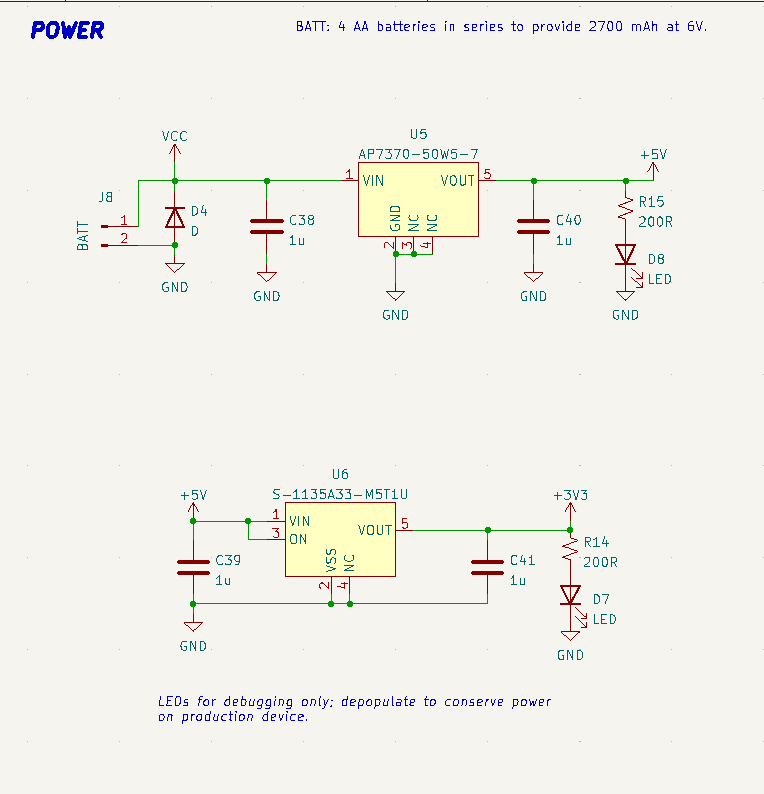
\includegraphics[width= 0.4\textwidth]{pwr_sch.png}
		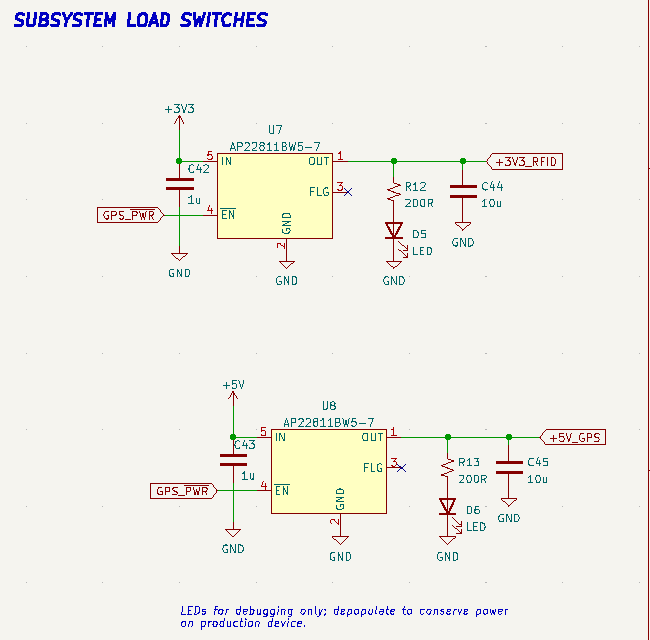
\includegraphics[width= 0.4\textwidth]{loadsw_sch.png}
		\caption{Power And Subsystem Load Switch Schematics.} \label{pwr_sch}
	\end{figure}
\end{center}


\textit{\textbf{Power Subsystem Requirements \& Verification:}}

\begin{figure}[H]
	\begin{center}
		\begin{tabular}{|p{0.3 \linewidth}|p{0.6 \linewidth}|}
			\hline
			Requirement & Verification  \\
			\hline
			\begin{enumerate}
				\item The power system will provide 3V3 +/- 0.4 mV to all subsystems that require 3V3, and 5V to the subsystems that require 5V. 
			\end{enumerate}  & \begin{enumerate} 
				\item A multimeter will be used to ensure the voltage and current are as specified at different points on the board.
			\end{enumerate}
			\\
			\hline
			\begin{enumerate}
				\item The power system will power the device for over 24 hours. 
			\end{enumerate}  & \begin{enumerate}
				\item Connect a multimeter/oscilloscope to measure the voltage at the battery terminals. 
				\item Record data every two hours over two 12 hour periods. 
				\item The data from the device will be read to ensure that the values were reasonably constant over time.
			\end{enumerate} \\
			\hline
			\begin{enumerate}
				\item The microcontroller can fully power off the GPS and RFID subsystems when not in use by turning off the load switches shown in Figure \ref{pwr_sch}. 
			\end{enumerate}  & \begin{enumerate}
				\item Flash a test program to the micrcontroller that toggles the control signals GPS\_~PWR and RFID\_~PWR. 
				\item Measure the output voltage on pin 1 of U7 and U8 to verify that the RFID and GPS subsystems are powered off. 
			\end{enumerate} \\
			\hline
		\end{tabular}
	\end{center}
	\caption{Power Subsystem R\&V Table.}
\end{figure}


\subsubsection{Alarm Subsystem} 

We will use a simple Piezo buzzer as the alarm. The alarm will be driven by the driver circuit shown in figure \ref{buzzer}. As shown in the diagram, when the FET is turned off, the circuit draws negligible current, thus minimizing power draw. 



\begin{center}
	\begin{figure}[H]
		\centering
		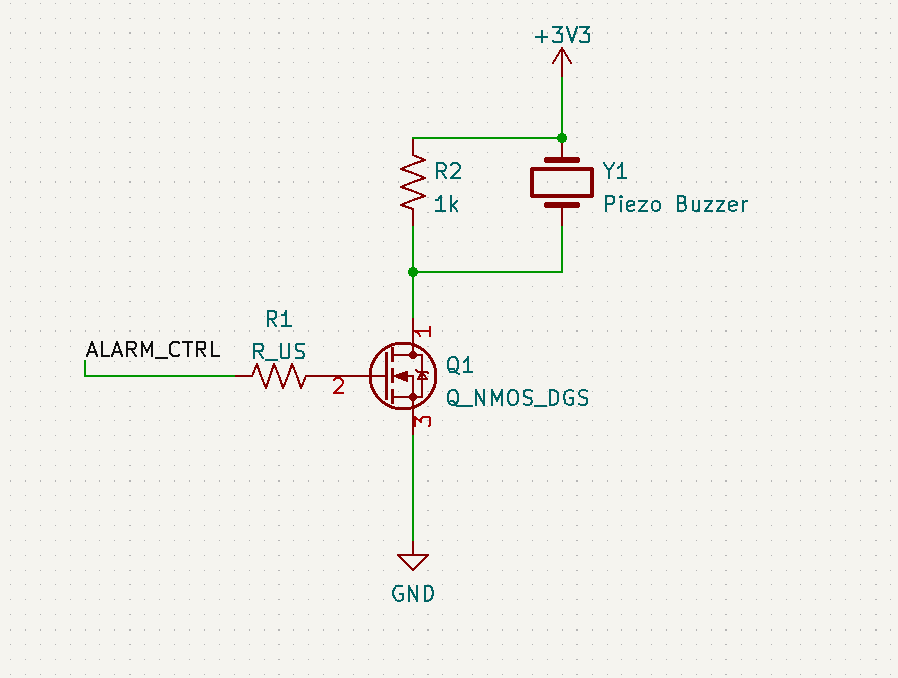
\includegraphics[width=0.25 \textwidth]{buzzer_ckt.png}
		\caption{Basic Piezo buzzer driver circuit.} \label{buzzer}
	\end{figure}
\end{center}


\paragraph{} 

\textit{\textbf{Alarm Subsystem Requirements \& Verification:}}


\begin{figure}[H]
	\begin{center}
		\begin{tabular}{|p{0.3 \linewidth}|p{0.6 \linewidth}|}
			\hline
			Requirement & Verification  \\
			\hline
			\begin{enumerate}
				\item The alarm makes noise when triggered by the ALARM\_CTRL signal. 
			\end{enumerate}  & \begin{enumerate}
				\item Flash a test program to the microcontroller that toggles the ALARM\_CTRL signal.
				\item Verify that when ALARM\_CTRL=1, the alarm makes noise. 
			\end{enumerate} \\
			\hline
			\begin{enumerate}
				\item The alarm circuit draws < 1 uA of current when not making noise.
			\end{enumerate}  & \begin{enumerate}
				\item Set ALARM\_CTRL to 0 through code.
				\item Use multimeter to measure voltage and current value from the alarm.
			\end{enumerate} \\
			\hline
		\end{tabular}
	\end{center}
	\caption{Alarm Subsystem R\&V Table.}
\end{figure}


\subsubsection{Base Station Subsystem} 

\paragraph{} 
Since we have limited resources for PCB development, our main PCB is designed such that it can be used for both the on-bike system and the base station receiver system with minor (and non-destructive) modifications (ie, jumpers and DNP components). Like the on-bike control board, the base station system will use the STM32WL55CC integrated transceiver and microcontroller to control the device and receive LoRa. We will use an FTDI I2C $\leftrightarrow$ USB IC to allow the microcontroller to communicate with the user's laptop -- the laptop will appear as an I2C slave device to the microcontroller, and the microcontroller will continously transfer data to the computer as the data is received. To increase ease of use, the base station will also be able to be powered over USB. 

On the computer, the user will be able to access the data via a GUI likely implemented in Python. The GUI will allow the user to access historical GPS data, and see recent GPS data plotted on a map. 

\begin{center}
	\begin{figure}[H]
		\centering
		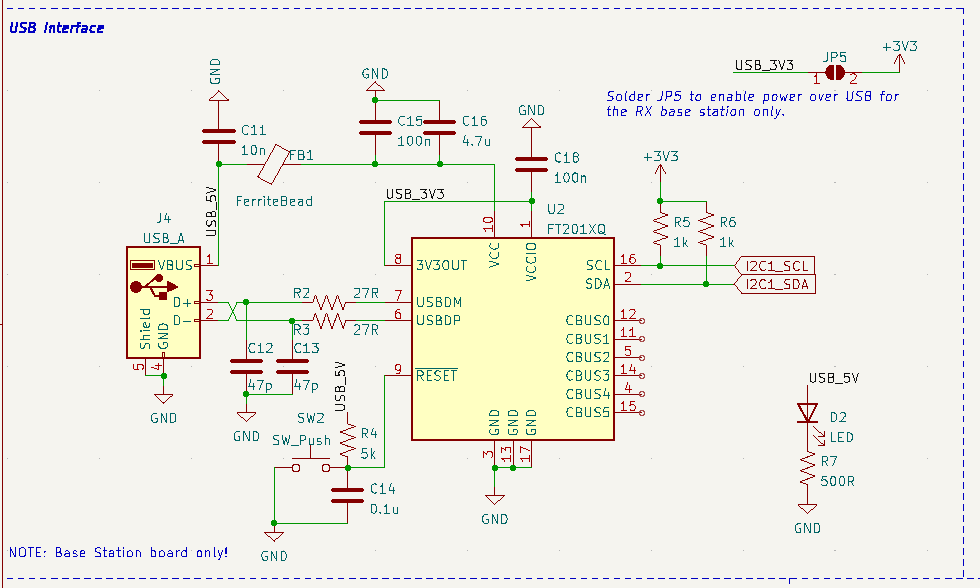
\includegraphics[width= \textwidth]{usb_interface.png}
		\caption{USB Interface Schematic.} \label{i2c_usb}
	\end{figure}
\end{center}

\paragraph{} 


\textit{\textbf{Base Station Subsystem Requirements \& Verification:}}

\begin{figure}[H]
	\begin{center}
		\begin{tabular}{|p{0.3 \linewidth}|p{0.6 \linewidth}|}
			\hline
			Requirement & Verification  \\
			\hline 
			\begin{enumerate}
				\item  The receiver board will interface with the computer over USB.
			\end{enumerate}  & \begin{enumerate}
				\item Flash a test program to the base station board that sends continuous data over the I2C/USB interface.
				\item Connect the base station board to the user computer and view the data sent over USB. 
				\item Verify the received data matches the sent data. 
			\end{enumerate} \\
			\hline
			\begin{enumerate}
				\item The receiver board will receive LoRa packets from the bike-based device. 
			\end{enumerate}  & \begin{enumerate}
				\item Flash a test program to the TX (bike system) board that transmits continuous data. 
				\item Flash a test program to the RX (base station) board that listens for data and continuously sends received data to the computer over I2C (USB to the computer). 
				\item Verify the data sent from the TX board is received by the RX board.
			\end{enumerate} \\
			\hline
			\begin{enumerate}
				\item The GUI will display GPS data over the past day, week, month, or year on a map. 
			\end{enumerate}  & \begin{enumerate}
				\item Flash a test program to the TX (bike system) board that transmits data with (false) timestamps that cover a 6-month period. 
				\item Transmit the data and receive it with the base station board. 
				\item Using the GUI, plot the data and verify the output plots match the data sent by the TX board. 
			\end{enumerate} \\
			\hline
			\begin{enumerate}
				\item The GUI will allow the user to view plots of the average speed and distance traveled.
			\end{enumerate}  & \begin{enumerate}
				\item Flash a test program to the TX (bike system) board that transmits data with (false) timestamps that cover a 6-month period. 
				\item Transmit the data and receive it with the base station board. 
				\item Using the GUI, plot the average speed and distance traveled and verify that it matches the data transmitted by the bike system board. 
			\end{enumerate} \\
			\hline

		\end{tabular}
	\end{center}
	\caption{Alarm Subsystem R\&V Table.}
\end{figure}


\subsection{Tolerance Analysis}\label{tol}

\paragraph{} 
Since this is a battery-powered device that is meant to be unattended for relatively long periods of time, it is critical that our power system can supply adequate power for the device over a period of time. Our battery pack will provide approximately 2700 mAh; since we will be using linear regulators, we can assume that the current drawn by the load is the same as the current drawn from the battery pack, and do the power calculation in terms of available milliamp-hours. (Refer to Section \ref{ughhhh} for an in-depth explanation of this shortcut). We must calculate the total current draw for our device to ensure the battery can provide enough power to power the device for an appropriate period of time. 

\begin{figure}[H]
	\begin{center}
		\begin{tabular}{|c|c|c|c|c|}
			\hline
			\textbf{Subsystem} &  \textbf{Current Drawn} & \textbf{Duty Cycle Estimate} \\
			\hline
			Microcontroller/LoRa, high power TX \cite{stm_datasheet} & 120 mA & 5 \% \\
			\hline
			Microcontroller/LoRa \cite{stm_datasheet}, Idle & 3.45 mA & 100 \% \\
			\hline 
			GPS module \cite{gps} & 50 mA & 100 \% \\
			\hline
			RFID module \cite{rfid} & 45 mA & 100 \% \\ 
			\hline 
			Alarm ON & 3.3 mA & 1 \% \\ 
			\hline
			
			
		\end{tabular}
	\end{center}
	\caption{Power Budget Analysis}
\end{figure}

From the chart above, we can see that the full current drawn during operation (assuming 100\% duty cycle for the RFID and GPS module) is: 

$$ 
120(0.05) \text{ mA}+ 3.45 \text{ mA}+ 50\text{ mA} + 45\text{ mA} + 3.3 \text{ mA}= 107.75 \text{ mA}
$$


Since the 3 AA batteries can provide 2700 mAh: 

$$ 
\frac{2700 \text{ mA}*\text{hours}}{107.75 \text{ mA} } = 25 \text{ hours of operation}
$$


This is acceptable, but ideally, the device would be able to autonomously operate for multiple days without being recharged. We can increase the operation time significantly by limiting the on-time of the RFID and GPS modules. With a duty cycle of 25 \% for both, we can increase the operational time, as shown below: 
\begin{figure}[H]
	\begin{center}
		\begin{tabular}{|c|c|c|c|c|}
			\hline
			\textbf{Subsystem} &  \textbf{Current Drawn} & \textbf{Duty Cycle Estimate} \\
			\hline
			Microcontroller/LoRa, high power TX \cite{stm_datasheet} & 120 mA & 5 \% \\
			\hline
			Microcontroller/LoRa \cite{stm_datasheet}, Idle & 3.45 mA & 100 \% \\
			\hline 
			GPS module \cite{gps} & 50 mA & 25 \% \\
			\hline
			RFID module \cite{rfid} & 45 mA & 25 \% \\ 
			\hline 
			Alarm ON & 3.3 mA & 1 \% \\ 
			\hline
			
			
		\end{tabular}
	\end{center}
	\caption{Power Budget Analysis: Decreased Duty Cycle}
\end{figure}
$$ 
120(0.05)\text{ mA} + 3.45\text{ mA} + 50(0.25) \text{ mA}+ 45(0.25) \text{ mA}+ 3.3 \text{ mA}= 36.5 \text{mA}
$$


$$ 
\frac{2700 \text{ mA}*\text{hours}}{36.5 \text{ mA} } = 74 \text{ hours of operation}
$$


74 hours of operation is still somewhat low, but more reasonable than a single day. As we proceed with the design, we will work to increase the operational time with a single charge even further by implementing power-saving measures on the device, adding another 3-cell battery pack in parallel, or using a higher-capacity battery. 


\section{Cost and Schedule}


\subsection{Cost Analysis}


\subsubsection{Materials}

\begin{figure}[H]
	\begin{center}
		\begin{tabular}{|c|c|c|c|c|c|}
			\hline
			\textbf{Part} &  \textbf{Description} & \textbf{Supplier} & \textbf{Part Number} & \textbf{Quantity} & \textbf{Cost (\$)} \\
			\hline
			ID-3LA (125 kHz)& RFID reader module & Sparkfun & SEN-11862 & 1 & 27.95 \\
			\hline
			EM-506 (48 channel) & GPS module & Sparkfun & GPS-12751 & 1 & 42.95 \\
			\hline
			STM32WL55CC & Microcontroller & Digikey & STM32WL55CCU6 & 1 & 11.20 \\
			\hline			
			MSO320SR & Piezo Buzzer & Digikey & 458-1369-ND & 1 & 7.88 \\
			\hline
			RFID Tag (125 kHz) & RFID Tag & Sparkfun & COM-14235 & 2
			 & 2.10 each \\
			 \hline
			Assorted Components & ICs, discrete passives,etc & Digikey &   &  & $\approx$ 50.0 \\
			\hline
			\textbf{Total} & & & & & \textbf{154.18} \\
			\hline
		\end{tabular}
	\end{center}
	\caption{Power Budget Analysis: Decreased Duty Cycle}
\end{figure}


\subsubsection{Labor}

For each engineer: 

\$42.07/hour * 2.5 * 120 hours = \$12,621 

Total for three engineers:

3* \$12, 621 = \$37, 863

\section{Ethics and Safety}
This project is designed with IEEE’s code of ethics in mind, and the main point as we work on the project is “to hold paramount the safety, health, and welfare of the public, to strive to comply with ethical design and sustainable development practices, to protect the privacy of others, and to disclose promptly factors that might endanger the public or the environment” \cite{ethics}.

A proponent safety concern among electrical design is the battery. With the consideration of including a rechargeable battery, proper use and design may lead to battery failure - potentially leading up to explosion. As such, we work to limit the risk by ensuring that the amount of power drawn and the cell voltage are maintained within the safety limit of the battery used through the use of a power regulator. We are also making sure that the design accounts for the battery being maintained and operated in safe operating conditions.
Battery Charge/Discharge?

Furthermore, the design is implemented with LoRa and RF identification, which involves the transmitting and receiving of information wirelessly. As such, an ethical consideration that is paramount to our objective is that data is received accurately. This is important because if given false or failed readings thieves can make off with the bike even with the flawed design attached due to failure or misreading of information. As such, we plan to ensure that the correct RFID tag can communicate with the appropriate transmitter such that the alarm will sound if and only if the bike is in motion and reaches out of range of the appropriate RFID. 

\subsection{Calendar}


\begin{figure}[H]
	\begin{center}
		\begin{tabular}{|p{0.05 \linewidth}|p{0.6 \linewidth}| p{0.2 \linewidth}| }
			\hline
			2/21 & \textbf{Design Document Due} & People \\
			\hline 
			2/28  & \textbf{PCB Review} \begin{enumerate}
				\item Finish completely designing PCB and review draft with Professor
				\item Order all parts necessary for project
			\end{enumerate} 
		 & Team \\
		 \hline 
		 3/7  & \textbf{1st Round PCB Order Due} \begin{enumerate}
		 	\item Edit according to any request made by Professor
		 	\item Start writing code for testing PCB
		 \end{enumerate} 
		 & \begin{enumerate}
		 	\item Elizabeth
		 	\item Alex, Srinidhi
		 \end{enumerate} \\
		 3/14  & \textbf{Spring Break} &  \\
		 \hline 
		 3/21  & \textbf{2nd Round PCB Order Due} \begin{enumerate}
		 	\item Solder all parts and test 1st draft of PCB circuit
		 	\item If not functional makes changes and submit 2nd draft of PCB
		 \end{enumerate} 
		 & \begin{enumerate}
		 	\item Srinidhi, Alex
		 	\item Elizabeth
		 \end{enumerate} \\
		 \hline 
		 3/28  & \textbf{Individual Progress Reports Due} \begin{enumerate}
		 	\item Code State Machine (Start writing code for subsystems)
		 	\item LoRa
		 	\item RFID, GPS
		 	\item Power, Alarm
		 \end{enumerate} 
		 & \begin{enumerate}
		 	\item Team
		 	\item Elizabeth
	 		\item Srinidhi
	 		\item Alex 
		 \end{enumerate} \\
		 \hline 
		 4/4  & \textbf{Finish Writing Code for all Subsystems
		 } \begin{enumerate}
		 	\item Write Control module code
		 	\item Write Receiver GUI Code
		 	\item Start Testing Code
		 \end{enumerate} 
		 & \begin{enumerate}
		 	\item Elizabeth, Srinidhi
		 	\item Alex
		 	\item All 
		 \end{enumerate} \\
	 	\hline 
	 	4/11  & \textbf{Verify System Functionality and Continue Debugging} 
	 	& Team \\
	 	\hline 
	 	4/18 & \textbf{Mock Demo} \begin{enumerate}
	 		\item Prepare demo and continue working on any issues
	 	\end{enumerate} & Team \\ 
 		\hline 
 		4/25 & \textbf{Demo} \begin{enumerate}
 			\item Work on final presentation and paper
 		\end{enumerate} & Team \\
 		\hline 
 		5/2 & \textbf{Final Paper Due/Presentation} & Team \\ 
 		\hline 
		\end{tabular}
	\end{center}
	\caption{Team Calendar}
\end{figure}



\section{Appendix A: Derivation of Power Budget Calculation Shortcut} \label{ughhhh} 

\paragraph{} 

\textit{In response to the course staff's confusion about our Tolerance Analysis during the Design Document Review, we include this brief derivation to justify the calculation. }

Our power budget calculation in section \ref{tol} makes use of an intuitive shortcut to both shorten the calculation of the power budget and increase the accuracy. This shortcut arises from the fact that a linear regulator, at its core, is simply a variable resistor controlled by a feedback regulator, as shown by the conceptual circuit below: \cite{AD-linreg}

\begin{center}
	\begin{figure}[H]
		\centering
		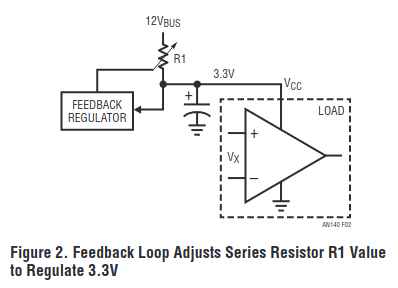
\includegraphics[width= 0.25 \textwidth]{linear_reg_diagram.png}
		\caption{Diagram from \cite{AD-linreg}} \label{linear_reg_diagram}
	\end{figure}
\end{center}

To calculate a power budget, we are interested in the efficiency ($eff = \frac{P_{load}}{P_{load} + P_{waste} } $)in the device. From the diagram we can see that the conceptual operation of the device is simply a resistor divider between R1 and the load, where R1 is varied by the feedback regulator to maintain a constant voltage across the load. Therefore, there are two sources of power dissipation ($P_{waste}$): the resistor R1, and the feedback network varying the resistance R1. The full power dissipated in the regulator can be trivially expressed as:

$$
P_{waste} = (I_{load} + I_{fb})*(V_{IN} - V_{OUT})+ I_{fb}*V_{OUT}. 
$$

In practice, the power dissipated in $R1$ is almost always several orders of magnitude greater than the power loss in the feedback regulator network, as the feedback regulator network is composed of switching devices and generally designed to minimize losses: $I_{load} >> I_{fb}$. To verify this, we can refer to the datasheets of devices that would be appropriate for our circuit (supplying 3V3 at up to 300 mA with a minimum dropout <1V). A cursory search on Digikey reveals many such models: the S-1135 Series has a quiescent current of 65 $\mu$A \cite{s-1135}, the NCP703 has a quiescent current of 12 $\mu$A \cite{ncp703}, and the NCP114 has a quiescent current of 50 $\mu$A \cite{ncp114}. 

Assuming a generously high current of 200 $\mu$A, a load current of 100 mA, and a generously low voltage drop from 4.5V to 3.3V, we can compare the solutions for power dissipation in two cases. Case 1 is the "true" calculation accounting for the losses due to both the quiescent current and the load current, in both R1 and the feedback network; Case 2 is the calculation assuming $I_{fb} \approx 0$ and the only loss is in R1. 

\textit{Case 1}: 
$$
P_{waste} = (I_{load} + I_{fb}) [A] * (4.5 - 3.3) [V]+ I_{fb} [A] * 3.3 [V] = 0.15096 [W]
$$

$$
eff = \frac{P_{load}}{P_{load} + P_{waste} } = 68.6\%
$$

\textit{Case 2}: 

$$
P_{waste} = I_{load} [A] * (4.5 - 3.3)[V] = 0.1503 [W]
$$

$$
eff = \frac{P_{load}}{P_{load} + P_{waste} } = 68.7\%
$$

The percent error as a result of using the approximation in case (2) is $ \frac{68.613 - 68.707}{68.613} = 0.14 \% $. Therefore, this approximation is extremely accurate in practical scenarios. 

\paragraph{}

We can rewrite the assumption in Case 2 as: 

$$
eff = \frac{P_{load}}{P_{load} + P_{waste} } = \frac{V_{o}* I_{o}}{V_{o}*I_{o} + (V_{i} - V_{o})*I_{i} }  \approx \frac{V_o}{V_i}
$$

Where $V_i$ is the voltage input to the regulator, $V_o$ is the voltage output of the regulator, and similarly $I_i$ is the curent into the regulator and $I_o$ is the current out of the regulator to the load. 

The amount of usable power from the battery is a conserved quantity, and can be expressed as in terms of the total power $P_{batt}$, the time $t$ in use, and the efficiency $eff$ as shown below. $P_{batt}$ can also be expressed as the commonly used current-time product (milliamp-hours) multipled by the battery voltage $V_i$. 
$$
E_{batt, usable} = P_{batt}*t*eff = (I_o*t)*V_i*eff
$$


Applying the assumption from Case 2:

$$
E_{batt,usable} = (I_{o} *t)* V_i \left( \frac{V_o}{V_i} \right) * t = (I_o*t)*V_o
$$

From this expression, \textit{the amount of energy available from the battery accounting for the linear regulator inefficiency} ($E_{batt, usable}$) is equivalent to \textit{the original specified output current-time product} $(I_o*t)$ multiplied by the output voltage of the linear regulator. 

To calculate a power budget, the following equation must be satisfied: 

$$
E_{batt, usable} = (I_o*t)*V_o \geq I_{load}* V_o * t_{operation}
$$

Dividing both sides by $V_o$: 

$$
(I_o*t) \geq I_{load}* t_{operation}
$$


Which is the equation we solved in section \ref{tol} to verify our power budget. Thus our calculation is valid, and, in fact, significantly more accurate than the suggestion to assume a blanket 60\% efficiency for all linear regulators. 



\begin{thebibliography}{}
	\bibitem{ethics} IEEE, "IEEE Code of Ethics," \textit{IEEE}, 2022 Available: https://www.ieee.org/about/corporate/governance/p7-8.html. [Accessed: Feb. 10 2022].
	\bibitem{LoRA} LoRa Alliance, "What is LoRaWAN: A Technical Overview of LoRa and LoRaWAN", 2015.
	
	\bibitem{gps} GlobalSat. "GlobalSat GPS Module Hardware Data Sheet." Product No: EM-506. 2013. https://cdn.sparkfun.com/datasheets/GPS/EM506\_um.pdf
	
	\bibitem{s-1135} Ablic. "S-1135 Series Voltage Regulator". 2018. https://www.ablic.com/en/doc/datasheet/voltage\_regulator/S1135\_E.pdf
	
	\bibitem{ncp703} ON Semiconductor. "300 mA, Ultra-Low Quiescent
	Current, IQ 12 uA, Ultra-Low Noise, LDO Voltage Regulator". https://www.onsemi.com/pdf/datasheet/ncp703-d.pdf.
	
	\bibitem{ncp114} ON Semiconductor. "NCP114/D Voltage Regulator - CMOS Low Dropout". 2020. https://www.onsemi.com/pdf/datasheet/ncp114-d.pdf. 
	
	\bibitem{rfid} ID-innovations. "ID-3LA, ID-12LA, ID-20LA Low Voltage Series Reader Modules." 2015. https://cdn.sparkfun.com/assets/c/7/0/e/3/DS-11828-RFID\_Reader\_ID-20LA\_\_125\_kHz\_.pdf
	
	\bibitem{reflector} Photograph by Julo, public domain, Wikimedia Commons Available: https://upload.wikimedia.org/wikipedia/commons/b/b1/BicycleRetroreflectors.JPG. [Accessed: Feb 10 2022]. 
	\bibitem{matchingAN} STMicroelectronics, "RF matching network design guide for STM32WL Series", AN5457, 2020. 
	
	\bibitem{stm_datasheet} STMicroelectronics, "Multiprotocol LPWAN dual core 32-bit Arm® Cortex®-M4/M0+	LoRa®, (G)FSK, (G)MSK, BPSK, up to 256KB Flash, 64KB SRAM", DS13293, 2021.
	
	
	\bibitem{battery} Wikipedia, "List of Battery Sizes", 2022. [Online]. Available: https://en.wikipedia.org/wiki/List\_of\_battery\_sizes. [Accessed: 10 Feb 2022]. 
	
	
	\bibitem{AD-linreg} Analog Devices, "Basic concepts of Linear Regulator and Switching Mode Power Supplies", Application Note 140, October 2013. 
\end{thebibliography}


\end{document}
